\chapter{Appendix: Monotonic Fairness Supplement}

In this supplement, we provide justification for our design choices for the neural network architecture, and demonstrate that such an architecture is able to capture monotonic functions, and impose monotonicity even when the true generating function is non-monotone.

\section{Design choices}
    Below, we discuss several design choices, and their effect on the resulting functions.

    \paragraph{Transformation Matters:} 
        The choice of transformation function in Equation 4 can have a significant effect on the probability of successful convergence of monotonic neural networks.  We show in Figure~\ref{fig:activations} that the choice of transformation can have different effects based on the nature of the underlying function, and affects both monotonic and non-monotonic fitting. We consider four non-linearities:
        \begin{itemize}
            \item Square: $\tau(x) = x^2$.
            \item Abs: $\tau(x) = |x|$.
            \item Offset exponential linear unit (elumod): \\$ \tau(x) = \left\{\begin{array}{c l} 
                    x       & ~\mbox{if}~ x > 1 \\ 
                    e^{x-1} & ~\mbox{if}~ x \le 1 \\ 
                \end{array}\right.$
            \item Softplus: $\tau(x) = \log(1+e^x)$
        \end{itemize}
        We choose to use an offset exponential linear unit in our experiments, since it achieved optimal or near-optimal convergence in these comparisons.
        
        \begin{figure}
            \centering
            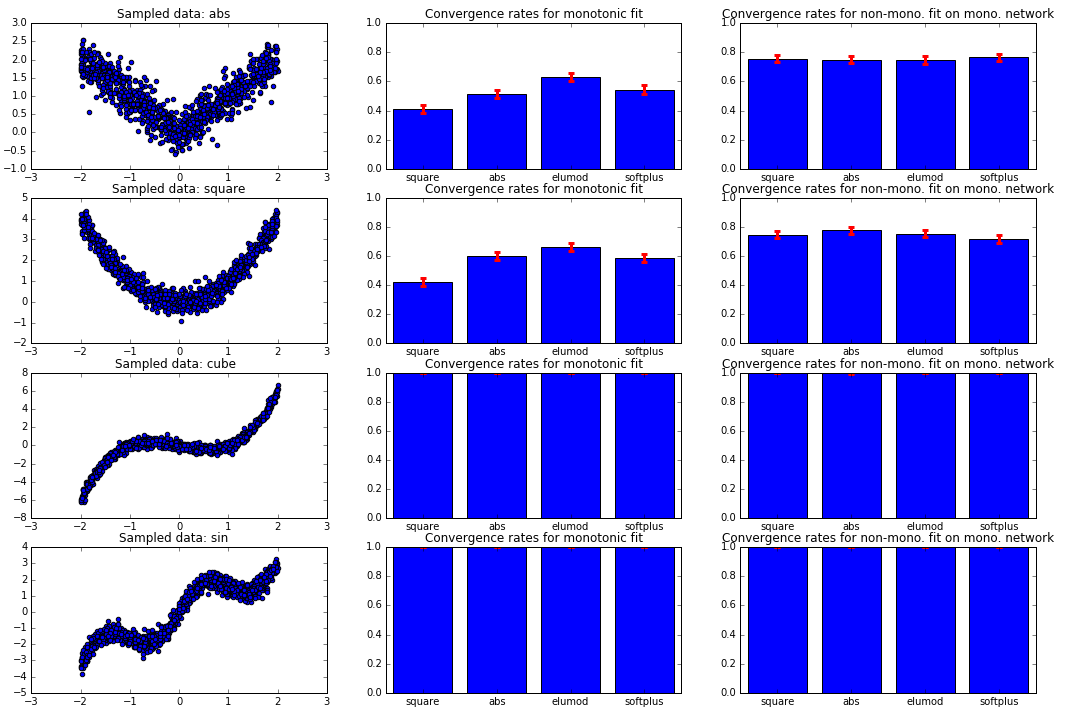
\includegraphics[width=\textwidth]{fig_monofair/activation_function_convergence.png}
            \caption{Convergence rates for various functions used to enforce positive weights. The vertical exist for the middle and right columns is the proportion of random initialization which converge to a non-deviant ($\hat{y} = \bar{y}$) solution.}
            \label{fig:activations}
        \end{figure}

    \paragraph{Activation Matters:} 
        Additional caution is needed in selecting an activation function for a monotonic neural network.  If, for instance, a convex activation function is used (e.g. \textit{elu} or \textit{relu}), subsequent layers can only compound this convexity, and the resulting function can only be convex.  It is easy to see this by considering the compounding of the first and second derivative across the layers.  This may be a desirable feature in some settings, but generally prohibits it from approximating \textit{any} monotonic function.  As such, bounded (but monotonic) activation functions like \textit{logistic} or \textit{tanh} are advisable for general purposes.
    
\section{Ability to Capture Mixed Monotonicity}

    We wish to emphasize that the network architecture described in this paper can simultaneously handle monotonic and non-monotonic relationships between the inputs and output. If we begin with the assumption that a network constrained to positive weights will produce a monotonically increasing function $f(x)$, we can briefly intuit the ability to fit a monotonically decreasing function by considering that $f(-x)$ would produce an identical function $f(x)$ but with reversed domain and therefore would be monotonically decreasing. Equivalently, we can enforce negativity on the weights in the network on edges leading out from any $x$ with respect to which $f(x)$ is monotonically decreasing, i.e. set $\tilde{w} < 0$ in the connection between $x$ and the first hidden layer (but keeping all weights in subsequent layers positive to maintain direction).  
    
    Further, if we accept that we can fit monotonically increasing and decreasing functions by constraining the weights, then consider what would happen if we fit $f(x, x)$, i.e. fed the same input twice, but constrained the first to be increasing and the second to be decreasing.  By the argument of decomposing functions into positive and negative parts (or, here, decomposing the first derivative into positive and negative parts), we can construct a monotonic function from its increasing and decreasing parts.  Further, each node in the first hidden layer would compute as $\sigma(\tilde{w}_{+} x + \tilde{w}_{-} x + c)$, which could be simplified as $\sigma(w x + c)$ where $w$ is unconstrained. 
    
    \begin{figure}
        \centering
        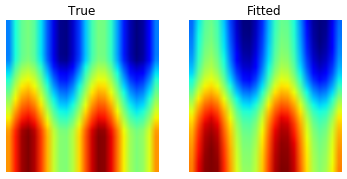
\includegraphics[width=.8\textwidth]{fig_monofair/mixed_monotonicity_demo_1.png}
        \caption{Demonstration of our network architecture's ability to fit a function which is monotonic in one dimension and non-monotonic in another. }
        \label{fig:demo1}
    \end{figure}
        
    To demonstrate the result empirically, we show in Figure~\ref{fig:demo1} a two-dimensional experiment in which the true underlying function is non-monotonic w.r.t to $x_1$ but strictly monotonically increasing w.r.t. $x_2$.  Specifically,
    $$ f(x_1, x_2) = \mbox{sin}(\pi x_1) + \mbox{max}(-1, \mbox{min}(1, x_2))  $$
    
    The estimated function shown is fit on a sample of 1,000 samples from the function and set to be non-monotonic w.r.t. $x_1$ and monotonic w.r.t $x_2$ and is able to recover the true function with reasonable precision.
    
    Similarly, we show in Figure~\ref{fig:demo2} that a mixed-monotonicity function can be fit even if the underlying function is severely non-monotonic (with the expected error in fit).  Here, $f(x_1, x_2) = x_0^2 + x_1^2$, and we again fit on a sample of 1,000 samples from the function and set to be non-monotonic w.r.t. $x_1$ and monotonic w.r.t $x_2$.  As expected, it finds a function which is optimal subject to the (incorrect) constraints.
    
    \begin{figure}
        \centering
        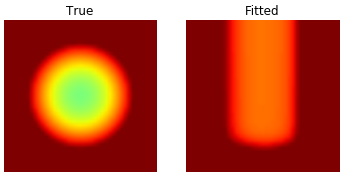
\includegraphics[width=.8\textwidth]{fig_monofair/mixed_monotonicity_demo_2.png}
        \caption{Demonstration of our network architecture's ability to created a function which is monotonic in one dimension and non-monotonic in another, even when the data does not meet those qualifications.}
        \label{fig:demo2}
    \end{figure}

